\chapter{Grundlagen}
In diesem Kapitel werden grundlegende Begriffe erklärt, die für das Verständnis der Arbeit unabdingbar sind.

\section{Cloud Computing}
Laut der Definition des National Institute of Standards and Technology (NIST), ist Cloud Computing ein Modell, dass einen einfachen on-demand Zugriff auf eine Menge von EDV Ressourcen ermöglicht, welche schnell und ohne Interaktion eines Service Providers bereitgestellt oder freigegeben werden können\cite{mell_nist_2011}.
Cloud Computing zeichnet sich demnach durch fünf Charakteristiken aus. Diese sind die bedarfsorientierte Bereitstellung von Ressourcen die durch einen Systembenutzer ausgelöst wird, den einfachen Zugriff über heterogene Plattformen hinweg durch standardisierte Netzwerkmechanismen, das Pooling von Servern und die schnelle und automatisierte Skalierung, scheinbar unendlich verfügbare Ressourcen und das dauerhafte Messen der Service Aktivitäten. \\
Darüber hinaus gehen aus der Definition verschiedene Servicemodelle hervor, die alle den Suffix "`as a service"', also "`als Dienstleistung"', gemeinsam haben. In der Definition des NIST werden die grundlegenden Servicemodelle IaaS, PaaS und SaaS genannt. Im weiterführenden ClouNS Referenz Modell\cite{kratzke_clouns_2016}, das in Abbildung \ref{fig:clouNS} zu sehen ist, werden sie um CaaS erweitert. \\

\begin{figure}[H]
    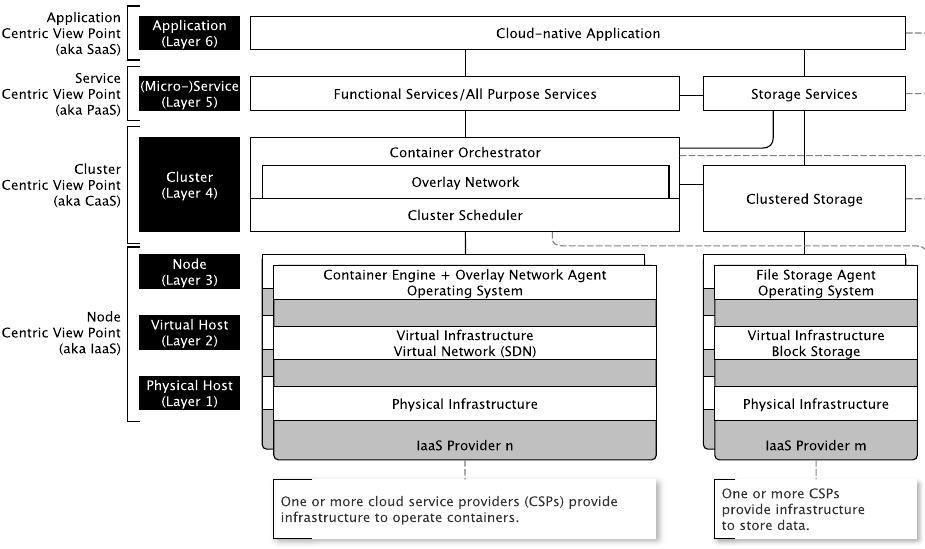
\includegraphics[width=\textwidth]{img/ClouNS_Stack.png}
    \caption[Der ClouNS Stack]{Der ClouNS Stack\cite{kratzke_clouns_2016}}
    \label{fig:clouNS}
\end{figure}

\subsection{Infrastructure as a Service (IaaS)}
Infrastructure as a Service bietet die Grundlage des Cloud Native Stacks. Einem Kunden werden hierbei grundlegende zumeist virtualisierte Hardware-Ressourcen wie Prozessorleistung, Speicher oder Netzwerkmöglichkeiten angeboten. Auf diesen kann er seine Software beliebig ausführen. Er hat Kontrolle über Betriebssysteme, Anwendungen und verwendeten Speicher seiner Instanzen\cite{mell_nist_2011}. \\

\subsection{Cluster-as-a-Service \ Container-as-a-Service (CaaS) }
Bei Cluster as a Service handelt es sich um eine Schicht über IaaS, die ein Clustering von Containern bietet. Hier agieren Orchestrierungs Tools wie zum Beispiel Kubernetes, die Container auf das Cluster verteilen, skalieren und managen\cite{kratzke_clouns_2016}. \\

\subsection{Platform as a Service (PaaS)}
PaaS liegt eine Ebene über IaaS oder CaaS. Einem Kunden wird auch hier die Kontrolle über die in der Cloud Infrastruktur auszuführende Anwendung gegeben. Allerdings kann er nicht über verwendete Betriebssysteme, Speichernutzung, Netzwerkkonfiguration usw. entscheiden. Dafür werden ihm vom Anbieter Programmier- oder Laufzeitumgebungen, Tools und Bibliotheken angeboten, die die Entwicklung und Ausführung der Anwendung auf der Infrastruktur ermöglichen\cite{mell_nist_2011}.\\

\subsection{Software as a Service (SaaS)}
SaaS ist eine höhere Abstraktionsebene über PaaS. Einem Kunden werden hier vom Anbieter explizite auf Cloud Infrastruktur auszuführende Anwendungen bereitgestellt, die dieser verwenden kann. Der Kunde hat weder Einfluss auf die zugrundeliegende Cloud Infrastruktur, noch auf verwendete Betriebssysteme oder Software. Die Ausnahme bilden limitierte Einstellungsmöglichkeiten der vom Anbieter bereitgestellten Anwendung\cite{mell_nist_2011}.

\section{Cloud Native Computing}
Cloud Native Technologien oder Cloud Native Computing ist laut der Cloud Native Computing Foundation (CNCF) eine Ansammlung von Technologien, die es Unternehmen ermöglichen "`skalierbare Anwendungen in modernen, dynamischen Umgebungen zu implementieren und zu betreiben"' \cite{noauthor_cncftoc_nodate}. Bei diesen dynamischen Umgebungen handelt es sich dabei ausschließlich um Cloud Umgebungen (also private, öffentliche und hybride Clouds). Diese Systeme sollen lose gekoppelt, "`belastbar, handhabbar und beobachtbar"' sein und durch Automatisierung schnelle Änderungen ermöglichen\cite{noauthor_cncftoc_nodate}.

\section{Containerisierung}
Containerisierung ist eine Technik, den Code einer Anwendung mitsamt aller Abhängigkeiten, die diese zur Ausführung benötigt, zu verpacken. Ein solches Paket wird als Container Image bezeichnet. Da alle Abhängigkeiten enthalten sind, werden dadurch die Laufzeitunterschiede auf unterschiedlichen Plattformen minimiert\cite{noauthor_what_nodate}. Zur Laufzeit wird ein Container Image als Container bezeichnet. Um ein Container Image auszuführen, wird eine Container Runtime benötigt. Die erste Container Runtime Engine wurde von Docker entwickelt, wird aber mittlerweile als Open-Source Projekt mit dem Namen containerd von der Open Container Initiative (OCI) betrieben\cite{noauthor_what_nodate}. 

Containerisierte Anwendungen unterscheiden sich von Virtuellen Maschinen vor allem darin, dass kein Hypervisor zur Ausführung der Images benötigt wird. Stattdessen teilen sich alle Container das Host-Betriebssystem und werden in einem eigenen User-Space isoliert. Dadurch können Container-Images deutlich leichtgewichtiger und schneller als Virtuelle Maschinen ausgeführt werden. Abbildung \ref{fig:containerVsVMs} verdeutlicht nochmals den Unterschied beider Technologien.

\begin{figure}[H]
    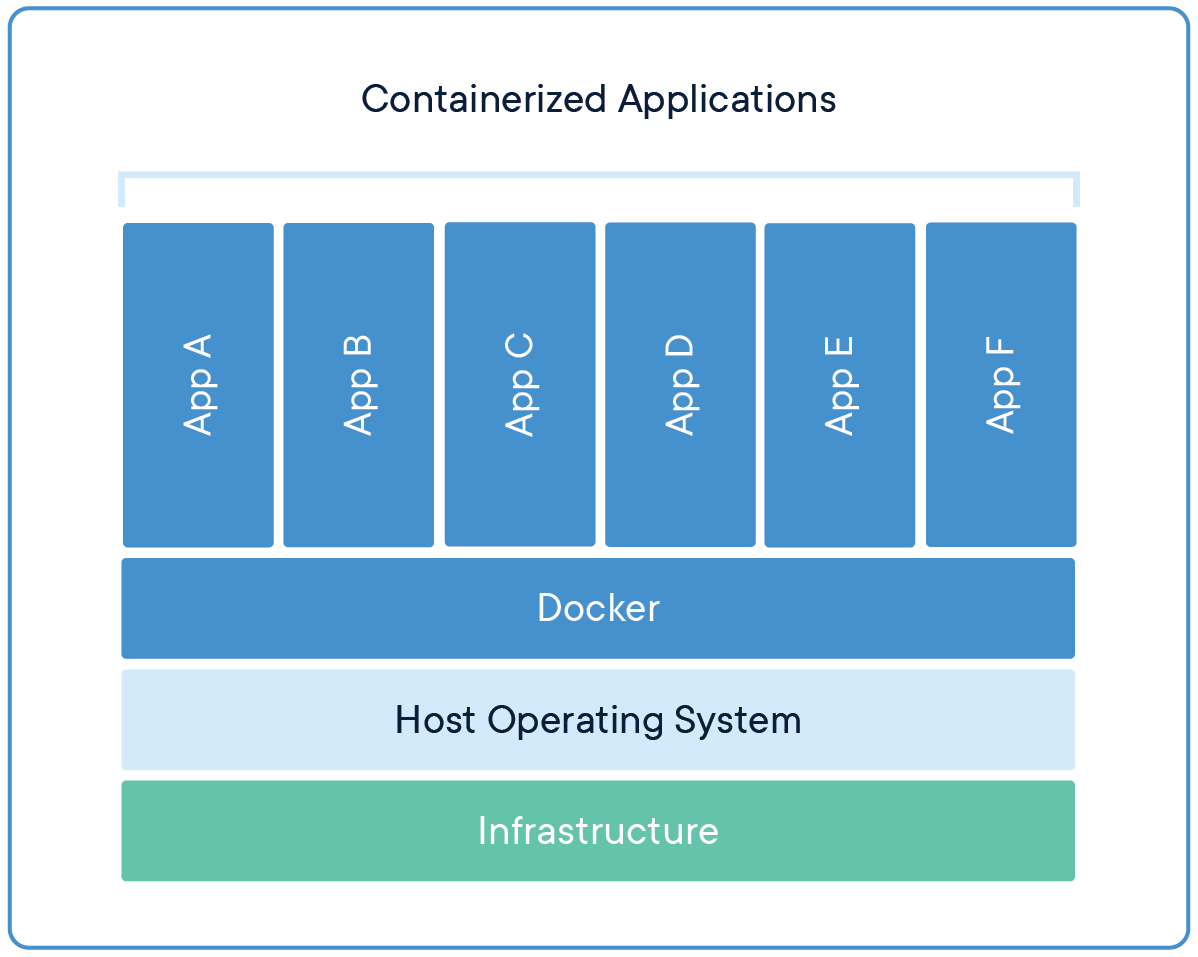
\includegraphics[width=200pt]{img/container-architecture.png}
    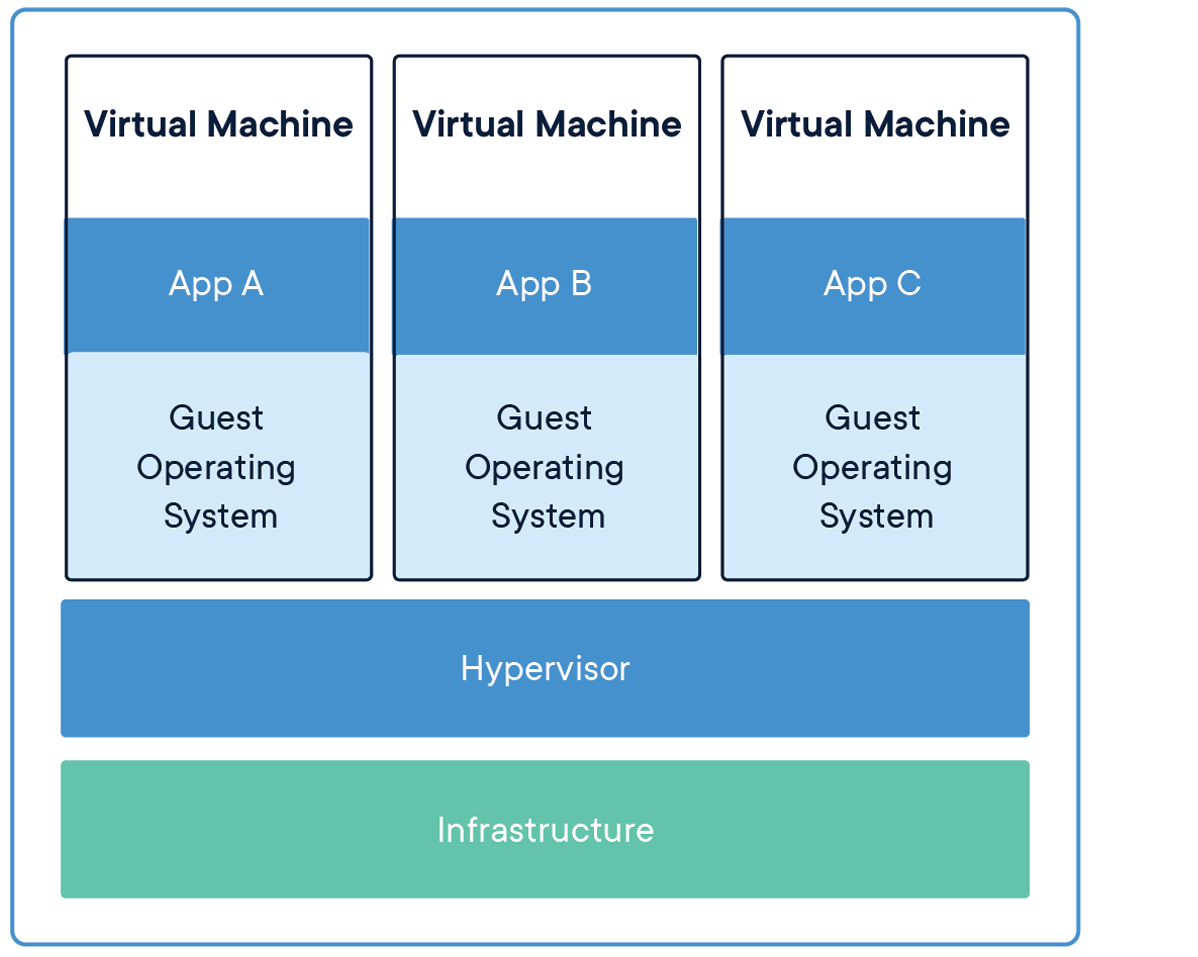
\includegraphics[width=200pt]{img/vm-architecture.png}
    
    \caption[Vergleich zwischen Containern und Virtuellen Maschinen]{Vergleich zwischen Containern und Virtuellen Maschinen\cite{noauthor_what_nodate}}
    \label{fig:containerVsVMs}
\end{figure}

\section{Container-Orchestrierung}
Container-Orchestrierung beschreibt die Automatisierung der "`Bereitstellung, Verwaltung, Skalierung und Vernetzung von Containern"'\cite{noauthor_was_nodate-1}. Mit Orchestrierungs-Tools lassen sich Container einfach auf Computer-Clustern provisionieren, skalieren und überwachen. Wie im ClouNS Modell (Abb. \ref{fig:clouNS}) zu sehen ist, agieren Container Orchestrierungs Tools auf der CaaS Ebene. Dadurch erlauben sie das Betreiben von infrastrukturunabhängigen und flexiblen Anwendungen auf Basis von Containern\cite{noauthor_was_nodate}. Beispiele für bekannte Orchestrierungs-Tools sind Kubernetes oder AWS Elastic Container Service (ECS).

\section{Serverless}
Serverless ist ein Software-Ausführungsmodell, bei dem ein Cloud Anbieter (z.B AWS, Azure, GCP) sich vollständig um die Ausführung einer Anwendung inklusive Konfiguration der zugrundeliegenden Server kümmert. Der Programmierer kann sich daher ausschließlich auf das Schreiben des Codes konzentrieren und muss keine Zeit in das Einstellen und Aufsetzen von Servern investieren.

Serverless Anwendungen werden grundlegend unterschieden in Functions-as-a-Service (FaaS) und Backends-as-a-Service (BaaS); wobei es sich bei letzterem um API-basierte, automatisch skalierte Services von Drittanbietern handelt, die grundlegende Bausteine einer Applikation ersetzen\cite{ken_owens_cncf_2018}. Beispiele für BaaS sind Amazon AWS Simple Storage Service (S3) als Speicher von Dateien oder AWS DynamoDB als NoSQL-Datenbank.

In dieser Arbeit sollen ausschließlich Functions-as-a-Service betrachtet werden. Dabei wird die Software in einem Stateless-Container, d.h einem Container ohne persistentem Speicher, ausgeführt. Der Cloud-Anbieter stellt dabei die Ressourcen dynamisch bzw. on-demand bereit, d.h die Anwendung wird nur dann ausgeführt, wenn eine diesbezügliche Anfrage eintrifft. Serverless verspricht dadurch eine effizientere Entwicklung und Kosteneinsparungen, da bei den Anbietern nur der tatsächlich laufenden Code abgerechnet wird\cite{noauthor_was_2016}. Im ClouNS Modell (Abb. \ref{fig:clouNS}) ist FaaS also eine Ebene über der von CaaS einzustufen, da es eine Plattform zur Entwicklung von Software darstellt, die Container und deren Orchestrierung als Basis nutzen.

\section{AWS Lambda}
Die in dieser Arbeit getestete Serverless-Anwendung wird auf AWS Lambda ausgeführt. Dabei handelt es sich um ein FaaS Angebot von Amazon AWS. Die Funktionsweise von Lambda lässt sich wie folgt beschreiben\cite{amazon_aws_aws_2020}:

\begin{enumerate}
\item Es tritt ein Event ein, dass die Ausführung der Lambda-Funktion anfordert. \\
    Dabei kann es sich um alle mögliche Ereignisse handeln. Zum Beispiel ein Dateiupload in S3, einen CRON-Job oder im Falle eines Web Backends eine API-Aufruf mittels AWS API-Gateway.

\item Init Phase: Lambda erstellt automatisch eine Ausführungsumgebung (environment). \\
    Dabei handelt es sich um eine isolierte Umgebung, die für die Ausführung der Lambda- Funktion benötigt wird. Für diese Umgebung lassen sich einige Parameter von Anwender konfigurieren:
    
    \begin{enumerate}
        \item Die Runtime: Dabei handelt es sich um die verwendete Programmiersprache bzw. Framework. Als Optionen bietet Lambda beispielsweise Node.js 12.x, Java, Python oder Go.
        \item Die Arbeitsspeichergröße: Wie viel Speicher der ausgeführten Funktion bereitsteht. Die Mindestgröße beträgt hier 128MB; maximal sind etwas mehr als 10GB möglich. Proportional zur Speichergröße bestimmt Lambda ebenfalls die CPU Leistung, mit der die Funktion ausgeführt wird.
        \item Timeout: Die maximale Ausführungszeit der Funktion bevor Lambda sie automatisch beendet. Hier sind maximal 15 Minuten möglich.
    \end{enumerate}
    
    Die Umgebung wird mit den konfigurierten Ressourcen (Speicher, CPU) erstellt, der Code der Funktion geladen und entpackt und der Initialisierungscode der Lambda Funktion (nicht die Funktion an sich) ausgeführt. Dort lässt sich bspw. eine Datenbankverbindung aufbauen.
    
\item Invoke Phase: In dieser Phase wird die eigentliche Lambda Funktion, welche auch als Handler bezeichnet wird, ausgeführt. Eventuelle Rückgabewerte werden an den Aufrufer zurückgeliefert. Nachdem der Handler ausgeführt wurde, bleibt er verfügbar für weitere Anfragen. Der Initialisierungscode wird allerdings nicht mehr ausgeführt.
    
\item Shutdown Phase: Nachdem die Funktion für einige Zeit nicht mehr angefragt wurde, wird die Ausführungsumgebung wieder freigegeben. 
\end{enumerate}

\begin{figure}[H]
    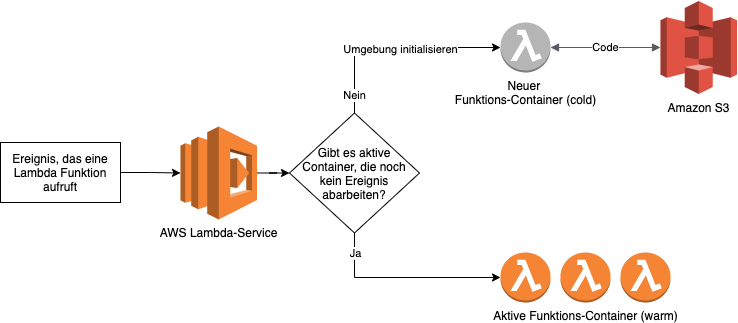
\includegraphics[width=\textwidth]{img/lambda-architecture.png}
    
    \caption[AWS Lambda Funktionsweise]{AWS Lambda Funktionsweise\cite{noauthor_serverless_2017}}
    \label{fig:lambda-architecture}
\end{figure}

\subsection{Cold- und Warmstart}
Nachdem der Handler in der Invoke-Phase ausgeführt wurde, wird die Ausführungsumgebung nicht sofort wieder freigegeben, sondern für einige Zeit vorgehalten, um weitere Anfragen schneller zu bearbeiten. Dies wird auch als Warmstart bezeichnet, da die Runtime-Umgebung bereits initialisiert ist und der Handler sofort aktiviert werden kann.
Muss die Umgebung nach einer eingetroffenen Anfrage erst noch initialisiert werden, also erst die Init-Phase ausgeführt werden, wird dies als Coldstart bezeichnet. Aufgrund des Mehraufwandes, erweist sich ein Coldstart als deutlich langsamer als ein Warmstart. Abbildung \ref{fig:lambda-architecture} verdeutlicht diesen Prozess.

\subsection{Nebenläufigkeit}
Befindet sich der Handler einer Lambda-Funktion gerade in der Ausführung und es trifft ein weiteres Ereignis ein, startet Lambda zusätzlich zu der bereits laufenden Funktion eine weitere Ausführungsumgebung, um diese neue Anfrage zu verarbeiten. Da nun mehrere Umgebungen gleichzeitig ausgeführt werden, wird dies auch als Nebenläufigkeit (engl. concurrency) bezeichnet. Bei vielen gleichzeitigen Anfragen werden also so viele Umgebungen wie nötig erstellt. Der AWS Lambda Service erlaubt standardmäßig 1000 nebenläufige Funktionen pro AWS Region, dieser Wert lässt sich allerdings nach Absprache mit AWS erhöhen.

Durch die Nebenläufigkeit wird die Stärke von Lambda Funktionen bei der Skalierung deutlich. Gibt es einen Anfragesturm, werden automatisch neue Instanzen aufgesetzt, die diese Bearbeiten können. Bereits initialisierte Umgebungen werden wiederverwendet. Lässt die Nachfrage nach, werden Umgebungen automatisch wieder heruntergefahren. 